\chapter{Lucrări Conexe}
\label{chap:ch2}

\par Acest capitol prezintă lucrările și metodele pe care se bazează soluția propusă. Sunt discutate, în ordine, calibrarea camerelor și corectarea distorsiunilor optice, metodele de estimare a adâncimii din imagini monoculare și multi-vizuale folosind modele bazate pe rețele neuronale, algoritmul RANSAC pentru filtrarea planului de mers din date ce conțin zgomot, precum și algoritmul A* pentru optimizarea traiectoriilor. Fiecare secțiune descrie principiile de funcționare ale metodelor relevante și modul în care acestea sunt utilizate sau adaptate în cadrul lucrării de față.

\section{Calibrarea Camerelor și Anularea Distorsiunilor}
\label{sec:ch2sec1}

\par Fundamentul oricărei analize metrice dintr-o imagine este stabilit prin calibrarea camerei. În lucrarea sa de referință \cite{zhang2000}, Zhang propune o tehnică flexibilă care a democratizat accesul la viziunea 3D prin eliminarea necesității unor aparate de calibrare costisitoare. Autorul demonstrează că utilizarea unui model plan (checkerboard) \ref{fig:figures/calib.io_checker_200x150_8x11_15.pdf} observat din cel puțin două orientări diferite este suficientă pentru a determina parametrii intrinseci și extrinseci ai camerei. Metoda se bazează pe calculul homografiei între planul modelului și proiecția sa în imagine, urmată de o rafinare neliniară prin criteriul verosimilității maxime care ia în considerare și distorsiunile radiale ale lentilei. Această abordare a transformat calibrarea dintr-un proces restrictiv de laborator într-o procedură aplicabilă în scenarii de utilizare reală.

\begin{figure}[htbp]
    \centering
    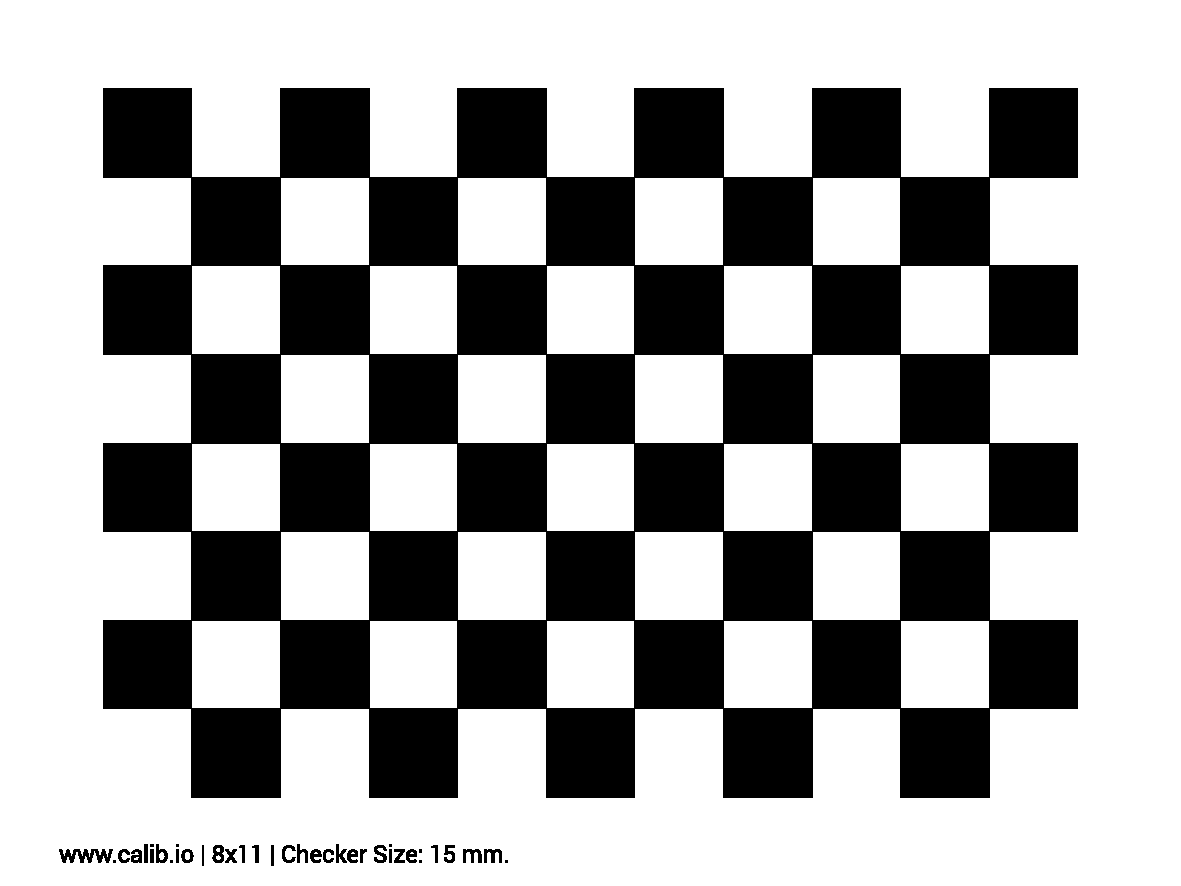
\includegraphics[width=0.8\linewidth]{figures/calib.io_checker_200x150_8x11_15.pdf}
    \caption{Exemplu de checkerboard pattern utilizat pentru a efectua calibrarea camerei, având 8 linii, 11 coloane(6 linii interne, 9 coloane interne) în care fiecare latură a unui pătrat măsoară 15 milimetrii pe o suprafață plană dreptunghiulară cu lungimea de 200 milimetrii, și lățimea de 150 de milimetrii, generat de platforma \url{https://calib.io}.}
    \label{fig:figures/calib.io_checker_200x150_8x11_15.pdf}
\end{figure}

Calibrarea estimează matricea $\mathbf{A}$ și coeficienții de distorsiune radială prin minimizarea erorii de reproiecție pe un set de imagini ale unui șablon de tip tablă de șah cu dimensiuni cunoscute. Soluția constă dintr-o estimare inițială în formă închisă, rafinată ulterior prin algoritmul Levenberg-Marquardt \cite{zhang2000}.

Parametrii obținuți sunt utilizați în două etape ale procesării. În primul rând, fiecare cadru este rectificat geometric pentru a elimina distorsiunile radiale ale obiectivului, asigurând consistența cu modelul pinhole \cite{hartley2004}. În al doilea rând, lungimea focală medie $f = (\alpha +
\beta)/2$ este utilizată pentru conversia ieșirii modelului de adâncime în metri, conform formulei \cite{depthanything3}:

\begin{equation}
    d_{\text{metric}} = \frac{f \cdot d_{\text{raw}}}{300}
\end{equation}

unde $d_{\text{raw}}$ reprezintă valoarea brută estimată de model, iar constanta $300$ provine din transformarea spațiului canonic al camerei utilizată în antrenarea modelului \cite{depthanything3}. În absența calibrării, lungimea focală este estimată presupunând un câmp vizual orizontal de $70°$, permițând funcționarea sistemului cu o precizie metrică redusă.

\section{Modele AI pentru Estimarea Adancimilor}
\label{sec:ch2sec2}

\par Odată stabilit modelul geometric, sarcina centrală devine inferarea adâncimii din imagini monoculare. Evoluția acestei sarcini este urmărită cel mai bine prin familia de modele \emph{Depth Anything}, prezentată în continuare în ordine cronologică.

\par Punctul de plecare îl reprezintă Depth Anything V1, introdus de Yang et al. \cite{yang2024depthv1} în cadrul conferinței Computer Vision and Pattern Recognition (CVPR) din 2024. Contribuția centrală a acestei lucrări nu constă într-un modul arhitectural nou, ci în scalarea masivă a datelor de antrenament: autorii proiectează un motor de date (\emph{data engine}) care colectează și etichetează automat aproximativ 62 de milioane de imagini neetichetate, alături de cele 1{,}5 milioane de imagini etichetate disponibile. Din punct de vedere arhitectural, modelul combină un encoder de tip DINOv2 \cite{oquab2024dinov2} cu un decodor DPT și estimează adâncime relativă de tip afin-invariant. Pentru ca volumul mare de date să fie valorificat, sunt propuse două strategii: impunerea unui obiectiv de optimizare mai dificil prin augmentări puternice, care forțează modelul să caute activ indicii vizuale suplimentare, și o supraveghere auxiliară care transferă priorii semantici bogați din encoderul preantrenat. Rezultatul este un model fundațional cu o capacitate de generalizare \emph{zero-shot} remarcabilă pe imagini din medii necunoscute, putând fi rafinat ulterior pentru adâncime metrică pe seturi precum NYUv2 \cite{silberman2012nyuv2} și KITTI \cite{geiger2012kitti}.

\par Construind direct peste acest fundament, Yang et al. \cite{yang2024depth} introduc Depth Anything V2, care schimbă sursa principală a supervizării: în locul imaginilor reale etichetate manual, antrenarea se bazează pe date sintetice, ale căror etichete de adâncime sunt absolut precise și permit învățarea detaliilor geometrice fine. Pentru a depăși decalajul de domeniu dintre imaginile sintetice și cele reale, V2 păstrează ideea scalării datelor din V1, dar o reorganizează într-o schemă de tip profesor-elev (\emph{teacher-student}): un model profesor de mare capacitate, antrenat exclusiv pe date sintetice, generează etichete pseudo-adâncime pe un volum masiv de imagini reale neetichetate, pe care apoi sunt antrenate modelele-elev. Față de V1, această modificare aduce hărți de adâncime mai robuste și cu o granularitate net superioară, în special în zonele cu structuri fine și obiecte transparente, păstrând în același timp o eficiență computațională ridicată.

Extinzând aceste capacități către o înțelegere multi-vizuală, Depth Anything 3 (DA3) \cite{depthanything3} propune o metodă de recuperare a spațiului vizual din orice număr de intrări, indiferent dacă poziția camerei este cunoscută sau nu. Contribuția majoră a DA3 constă în demonstrarea faptului că o arhitectură simplă, bazată pe un transformator standard (vanilla DINO), este suficientă pentru a obține rezultate de ultimă oră fără a fi nevoie de specializări arhitecturale complexe. Prin utilizarea unui target de predicție de tip „depth-ray”, modelul reușește o consistență spațială remarcabilă, depășind standardele anterioare în acuratețea geometrică și în estimarea poziției camerei cu peste 23\% față de predecesorii săi.

\par Pentru a sintetiza evoluția celor trei generații, Tabelul~\ref{tab:da_params} compară dimensiunea modelelor, iar Tabelul~\ref{tab:da_perf} rezumă performanța în estimarea adâncimii relative (zero-shot) și metrice. La nivel de capacitate, se observă că abia V2 introduce varianta uriașă (\emph{Giant}, $\sim$1,3 miliarde de parametri), folosită ca model profesor, în timp ce DA3 menține aceeași gamă de dimensiuni, dar cu un backbone ușor mai compact. În privința metricilor clasice de adâncime, valorile sunt aproape identice între V1 și V2: progresul real al V2 se manifestă în detaliile fine și robustețe, aspecte care, așa cum notează chiar autorii \cite{yang2024depth}, nu sunt surprinse de aceste benchmark-uri standard. DA3 \cite{depthanything3} aduce câștiguri vizibile mai ales pe seturi precum ETH3D și își concentrează evaluarea pe acuratețea geometrică și pe estimarea poziției camerei, motiv pentru care nu raportează rezultate metrice monoculare în același format ca predecesorii.

\begin{table}[htbp]
    \centering
    \begin{tabular}{lccc}
        \toprule
        Variantă (encoder) & V1 & V2 & DA3 \\
        \midrule
        Small (ViT-S) & 24,8M & 24,8M & 22M \\
        Base (ViT-B)  & 97,5M & 97,5M & 86M \\
        Large (ViT-L) & 335,3M & 335,3M & 300M \\
        Giant (ViT-g) & --- & 1,3B & 1,13B \\
        \bottomrule
    \end{tabular}
    \caption{Numărul de parametri pentru variantele celor trei generații \emph{Depth Anything} \cite{yang2024depthv1, yang2024depth, depthanything3}. \emph{Notă:} pentru V1 și V2 cifrele provin din depozitele oficiale și includ modelul complet (encoder DINOv2 + decodor DPT), în timp ce pentru DA3 valorile raportate corespund în principal backbone-ului DINOv2; numerele nu sunt, prin urmare, măsurate identic.}
    \label{tab:da_params}
\end{table}

\begin{table}[htbp]
    \centering
    \begin{tabular}{lccccc}
        \toprule
         & \multicolumn{2}{c}{V1} & \multicolumn{2}{c}{V2} & DA3 \\
        \cmidrule(lr){2-3}\cmidrule(lr){4-5}\cmidrule(lr){6-6}
        Set de date & AbsRel$\downarrow$ & $\delta_1\uparrow$ & AbsRel$\downarrow$ & $\delta_1\uparrow$ & $\delta_1\uparrow$ \\
        \midrule
        \multicolumn{6}{l}{\textit{Estimare relativă (zero-shot)}} \\
        KITTI  & 0,076 & 0,947 & 0,074 & 0,946 & 0,953 \\
        NYU    & 0,043 & 0,981 & 0,045 & 0,979 & 0,974 \\
        Sintel & 0,458 & 0,760 & 0,487 & 0,752 & 0,755 \\
        ETH3D  & 0,127 & 0,882 & 0,131 & 0,865 & 0,986 \\
        DIODE  & 0,066 & 0,952 & 0,066 & 0,952 & 0,954 \\
        \midrule
        \multicolumn{6}{l}{\textit{Estimare metrică (fine-tuned)}} \\
        NYUv2  & 0,056 & 0,984 & 0,056 & 0,984 & --- \\
        KITTI  & 0,046 & 0,982 & 0,045 & 0,983 & --- \\
        \bottomrule
    \end{tabular}
    \caption{Performanța în estimarea adâncimii (encoder ViT-L), AbsRel ($\downarrow$, mai mic e mai bun) și $\delta_1$ ($\uparrow$, mai mare e mai bun). Rezultatele V1/V2 provin din \cite{yang2024depthv1, yang2024depth}, iar coloana $\delta_1$ pentru DA3 din \cite{depthanything3} (Tabel~4, reevaluare monoculară). \emph{Notă:} DA3 raportează doar $\delta_1$ pentru adâncimea relativă și nu publică rezultate metrice monoculare în acest format, de unde marcajul „---”.}
    \label{tab:da_perf}
\end{table}

\section{Filtrarea Planului de Mers}
\label{sec:ch2sec3}

\par În procesarea datelor extrase din mediul vizual, prezența zgomotului și a erorilor sistematice este inevitabilă. Fischler și Bolles \cite{10.1145/358669.358692} au introdus algoritmul RANSAC (Random Sample Consensus) ca o soluție pentru potrivirea modelelor matematice pe seturi de date ce conțin un procent ridicat de erori brute (outliers). Spre deosebire de tehnicile de tip „least squares”, RANSAC utilizează un proces iterativ de selecție a unui subset minim de date pentru a genera un model candidat, verificând apoi consensul acestuia cu restul datelor. Această paradigmă este vitală în analiza imaginilor, unde detectorii de trăsături pot genera corespondențe eronate; RANSAC permite izolarea modelului corect (cum ar fi un plan sau o poziție a camerei) prin ignorarea zgomotului care nu se conformează structurii geometrice globale.

\section{Optimizarea Traiectoriilor}
\label{sec:ch2sec4}

\par În final, având o reprezentare stabilă a spațiului și a obstacolelor, problema deplasării este redusă la găsirea unui drum optim. Hart et al. \cite{4082128} au oferit baza formală pentru determinarea căilor de cost minim prin algoritmul A*. Acesta utilizează o funcție euristică pentru a ghida procesul de căutare într-un graf, evaluând fiecare nod prin suma dintre costul parcurs de la start ($g$) și costul estimat până la țintă ($h$). Autorii demonstrează că dacă euristica $h$ este admisibilă (adică nu supraestimează niciodată costul real), algoritmul A* garantează găsirea căii optime. Această cercetare a stabilit echilibrul matematic între eficiența căutării și certitudinea soluției, rămânând o piatră de temelie pentru orice sistem de navigație care operează în spații de stare complexe.
